\subsection{Analyse von den Resultaten der «Fussabdrücke»}
Der Fragebogen von WWF zeigt auf wie viele Planeten man bräuchte wenn alle Menschen denselben Lebensstill hätten, wie derjenige der diesen Fragenbogen ausfüllt. Bei unserer Gruppe lagen die Werte zwischen 2,2 und 2,9. Der Durchschnitt liegt bei 2,575. Dies bedeutet das unser durchschnittlicher Lebensstill ungefähr 2,5 Erden bräuchte.
Interessant zu sehen ist das alle der Mitglieder genau gleich viel Energie verbrauchen in den öffentlichen Diensten und dies entsprich nur ein wenig mehr als der Idealwert, bei welchen wir nur eine Erde brauchen. Bei der Mobilität, Konsum, Wohnen und Ernährung liegen alle Mitglieder unserer Gruppe im x-fachen Bereich über dem Idealwert. Bei diesen Bereichen besteht das grösste Verbesserungspotenzial. Bei der Mobilität kann man unteranderem auf einen Auslandflug verzichten. Den eine Stunde im Flugzeug entspricht circa einem Monat Autofahren. 
Ebenfalls kann man auch bei der Ernährung sich einfach verbessern. Man sollte versuchen vor allem regionale Produkte zu konsumieren. Ebenfalls ist Fleisch verzehren eine grosse Belastung für die Umwelt, dies kann jedoch simpel reduziert werden in dem man den Verzehr reduziert oder gar ganz weglässt. Was uns in der Gruppe generell erstaunt hat ist die Tatsache das Eier und Milchprodukte die Umwelt ebenfalls sehr belasten. 
Mit ein mehr Aufwand, aber ebenfalls mit grossen Potenzial, ist eine Energieeinsparung bei dem Bereich Wohnen. Eine radikale aber sehr gute Option ist es das Auswechseln einer Ölheizung zu beispielsweise einer Pelletheizung, welche einiges Umweltfreundlicher ist. Desweitern besteht auch im kleineren Aufwand Verbesserungspotenzial, beispielsweise bei den Geräten die man benutzt, sollte man darauf achten das diese in einer guten Energieklasse bewertet sind. 
Als Abschluss kann man sagen das unsere Gruppe zwar klar unter dem schweizerischen Durchschnitt liegt aber dennoch einiges machen kann um die Belastung an der Umwelt zu verringern. 

\subsection{Einkaufsverhalten}

Zur Untersuchen des Konsumverhaltens wurden vorgängig unabhängig von der Gruppe Daten erfasst zu dem Konsumverhalten der einzelnen Studenten. Genauer gesagt wurde über eine Woche untersucht, von wo die Lebensmittel genau bezogen werden. Durch das Analysieren der Daten resultiere die Grafik. Daraus ist klar ersichtlich das der Grossteil der Produkte von Grosshändler wie Migros und Coop bezogen werden.
 \begin{figure}[H]
	\centering
	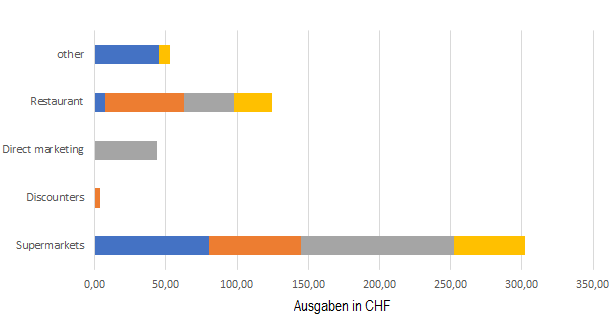
\includegraphics[width=0.9\textwidth]{ta}
	\caption{Analyse des Einkaufverhalten der einzelnen Studierenden}
\end{figure}
Diskussionen in der Gruppe hat ergab das die Hauptgründe dafür vor allem die Verfügbarkeit und die grosse Auswahl ist. Es kristallisierte sich heraus, dass die durch die Analyse der Auswahl von den verfügbaren Quellen ist, vor allem der Aspekt das Migros und Coop mittlerweile sehr viel regionale und nachhaltige Produkte im Sortiment vertreten sind ins Auge gefallen. Somit ist  das Streben nach Nachhaltigkeit nicht nach der frage, wo wir einkaufen, sondern was wir einkaufen zu klären, weil die Art der Produkte ein viel grösserer Einfluss darauf hat.